% !TEX root = ../main.tex
\section{实验\chinese{section}}
\subsection{实验题目}
UCS实验
\subsection{实验目的}
设置DCO FLL reference =ACLK=LFXT1 = 32768Hz, MCLK = SMCLK = 8MHz,输出ACLK、SMCLK,用示波器观察并拍照。
\subsection{实验仪器和设备}
计算机、开发板、示波器、信号源、电源、Code Composer Studio v5、串口调试助手等。
\subsection{实验步骤}
\begin{lstlisting}[language=C]
/****************************************
  |     XIN|-+
  |        | 32kHz
  |    XOUT|-+
  |   XT2IN|-+
  |        | 4mHz
  |  XT2OUT|-+
  |    P1.0|-->ACLK= 32,768Hz
--|RST P3.4|-->SMCLK= 8,000,000Hz
****************************************/
\end{lstlisting}
\par\indent 关闭看门狗,设置ACLK和SMCLK输出引脚,打开外部晶振使能。分别将P1.0和P3.4连接至示波器,观察波形分别为32768Hz和8MHz。
\subsection{程序清单}
\lstinputlisting{src/code/UCS.c}
\clearpage
\subsection{实验结果记录与分析}
\begin{figure}[htbp]
	\centering
	\begin{minipage}[htbp]{7.5cm}
		\centering
		\caption{UCS, ACLK}
		\label{UCS1}
		\includegraphics[width=7.5cm]{bitmap/bmp/UCS1.bmp}
	\end{minipage}
	\begin{minipage}[htbp]{7.5cm}
		\centering
		\caption{UCS, SMCLK}
		\label{UCS2}
		\includegraphics[width=7.5cm]{bitmap/bmp/UCS2.bmp}
	\end{minipage}
\end{figure}
\subsection{遇到的问题与解决方法}
\begin{enumerate}
	\item 一开始没有理解DCORSEL的用途,导致频率始终在范围的上限,无法输出8MHz;
	\item 在从示波器获取数据时遇到了一点麻烦。电脑上装的可以跟示波器通讯的上位机软件OpenChoice需要TekVISA串口软件。但TekVISA的驱动gadget serial v2.4有问题。一直显示该驱动未正确安装。很奇怪。凭着自己以前有过NI的MAXVISA的使用经历捣鼓了一会,没有成功;
	\item 于是改用U盘读取数据。但U盘读取数据时,明明显示"device successfully saved",但是将U盘插入电脑后却没有任何文件。搜索到了该示波器的说明书,但也没有帮助。之后在1个论坛里看到有用户反映示波器的存储格式非常老,想到可能是U盘的文件格式过新不支持的缘故。将U盘从NTFS格式化到exFAT仍旧不行。再将64GB的U盘分区到4GB格式化为FAT32才行(FAT32只支持4GB文件存储空间)。算是今天晚上一个非常有趣的收获了。
\end{enumerate}
\begin{figure}[htbp]
	\centering
	\begin{minipage}[htbp]{7.5cm}
		\centering
		\caption{TekVISA}
		\label{TekVISA}
		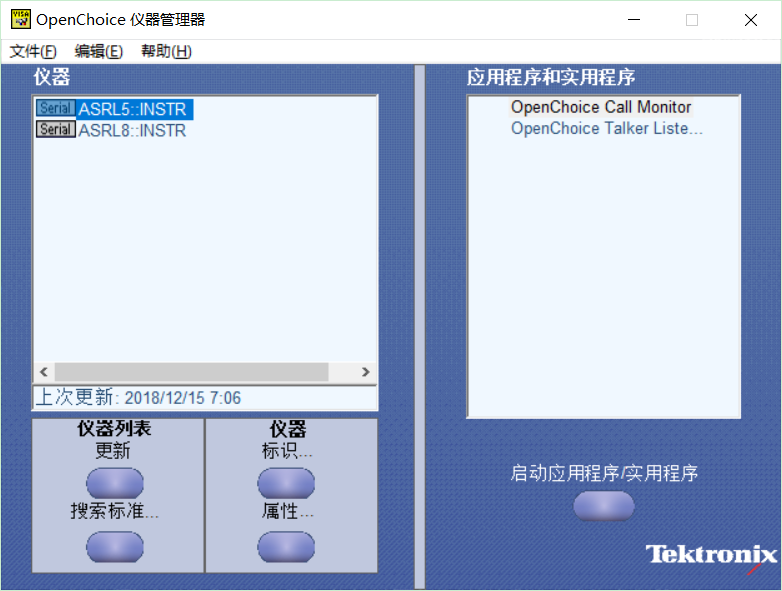
\includegraphics[width=7.5cm]{bitmap/png/TekVISA.png}
	\end{minipage}
	\begin{minipage}[htbp]{7.5cm}
		\centering
		\caption{OpenChoice}
		\label{OpenChoice}
		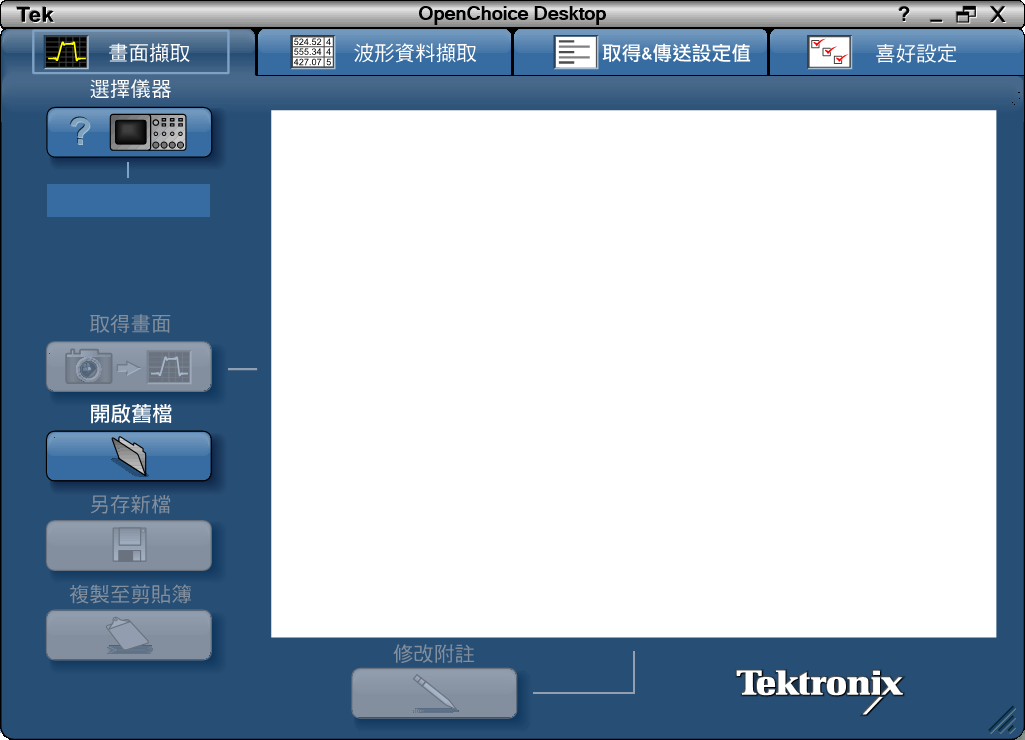
\includegraphics[width=7.5cm]{bitmap/png/OpenChoice.png}
	\end{minipage}
\end{figure}
